\documentclass[]{article}
\usepackage{lmodern}
\usepackage{amssymb,amsmath}
\usepackage{ifxetex,ifluatex}
\usepackage{fixltx2e} % provides \textsubscript
\ifnum 0\ifxetex 1\fi\ifluatex 1\fi=0 % if pdftex
  \usepackage[T1]{fontenc}
  \usepackage[utf8]{inputenc}
\else % if luatex or xelatex
  \ifxetex
    \usepackage{mathspec}
  \else
    \usepackage{fontspec}
  \fi
  \defaultfontfeatures{Ligatures=TeX,Scale=MatchLowercase}
\fi
% use upquote if available, for straight quotes in verbatim environments
\IfFileExists{upquote.sty}{\usepackage{upquote}}{}
% use microtype if available
\IfFileExists{microtype.sty}{%
\usepackage{microtype}
\UseMicrotypeSet[protrusion]{basicmath} % disable protrusion for tt fonts
}{}
\usepackage[margin=1in]{geometry}
\usepackage{hyperref}
\hypersetup{unicode=true,
            pdfborder={0 0 0},
            breaklinks=true}
\urlstyle{same}  % don't use monospace font for urls
\usepackage{graphicx,grffile}
\makeatletter
\def\maxwidth{\ifdim\Gin@nat@width>\linewidth\linewidth\else\Gin@nat@width\fi}
\def\maxheight{\ifdim\Gin@nat@height>\textheight\textheight\else\Gin@nat@height\fi}
\makeatother
% Scale images if necessary, so that they will not overflow the page
% margins by default, and it is still possible to overwrite the defaults
% using explicit options in \includegraphics[width, height, ...]{}
\setkeys{Gin}{width=\maxwidth,height=\maxheight,keepaspectratio}
\IfFileExists{parskip.sty}{%
\usepackage{parskip}
}{% else
\setlength{\parindent}{0pt}
\setlength{\parskip}{6pt plus 2pt minus 1pt}
}
\setlength{\emergencystretch}{3em}  % prevent overfull lines
\providecommand{\tightlist}{%
  \setlength{\itemsep}{0pt}\setlength{\parskip}{0pt}}
\setcounter{secnumdepth}{0}
% Redefines (sub)paragraphs to behave more like sections
\ifx\paragraph\undefined\else
\let\oldparagraph\paragraph
\renewcommand{\paragraph}[1]{\oldparagraph{#1}\mbox{}}
\fi
\ifx\subparagraph\undefined\else
\let\oldsubparagraph\subparagraph
\renewcommand{\subparagraph}[1]{\oldsubparagraph{#1}\mbox{}}
\fi

%%% Use protect on footnotes to avoid problems with footnotes in titles
\let\rmarkdownfootnote\footnote%
\def\footnote{\protect\rmarkdownfootnote}

%%% Change title format to be more compact
\usepackage{titling}

% Create subtitle command for use in maketitle
\newcommand{\subtitle}[1]{
  \posttitle{
    \begin{center}\large#1\end{center}
    }
}

\setlength{\droptitle}{-2em}

  \title{}
    \pretitle{\vspace{\droptitle}}
  \posttitle{}
    \author{}
    \preauthor{}\postauthor{}
    \date{}
    \predate{}\postdate{}
  
\usepackage{float}

\begin{document}

\begin{centering}

\vspace*{5 cm}

\Huge

{\bf Descubrimiento del Conocimiento usando herramientas de Big Data Módulo 2}

\vspace{3 cm}

\Large
Marco Andrés Vázquez Hernández

\vspace{1 cm}
\normalsize
Practica Estructura de la Información en redes. 

Septiembre de 2018

\normalsize
Instituto Politécnico Nacional


\end{centering}

\newpage

\section{Descripción}\label{descripcion}

Utilizando la herramienta y los datos trabajados en clase encontrar:

1.- La moduladidad de cada libro (guardar la grafica)

2.- El pagerank de cada libro (guardar la grafica)

3.- La representación del grafo visualmente (pdf)

\section{Libro 1}\label{libro-1}

\subsection{Moularidad, Pagerank y
Grafo}\label{moularidad-pagerank-y-grafo}

Modularity: 0.514\\
Modularity with resolution: 0.514\\
Number of Communities: 8

\begin{figure}[htbp]  
\centering
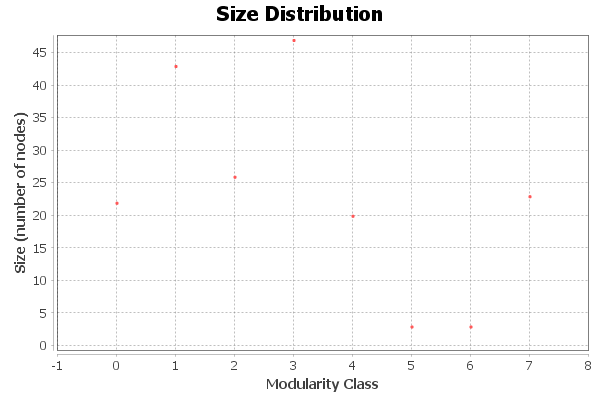
\includegraphics{modb1/communities-size-distribution.png}
\end{figure}

\begin{figure}[htbp]  
\centering
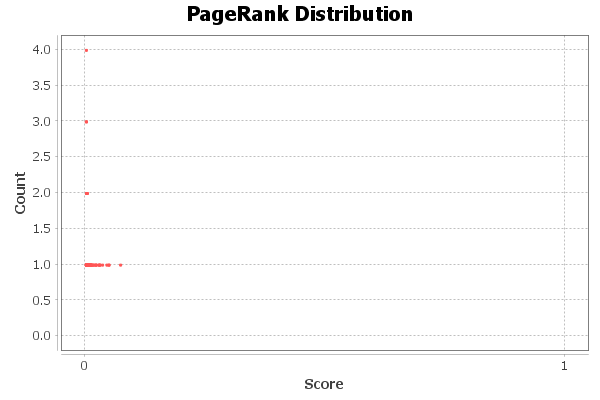
\includegraphics{prb1/pageranks.png}
\end{figure}

\begin{figure}[htbp]  
\centering
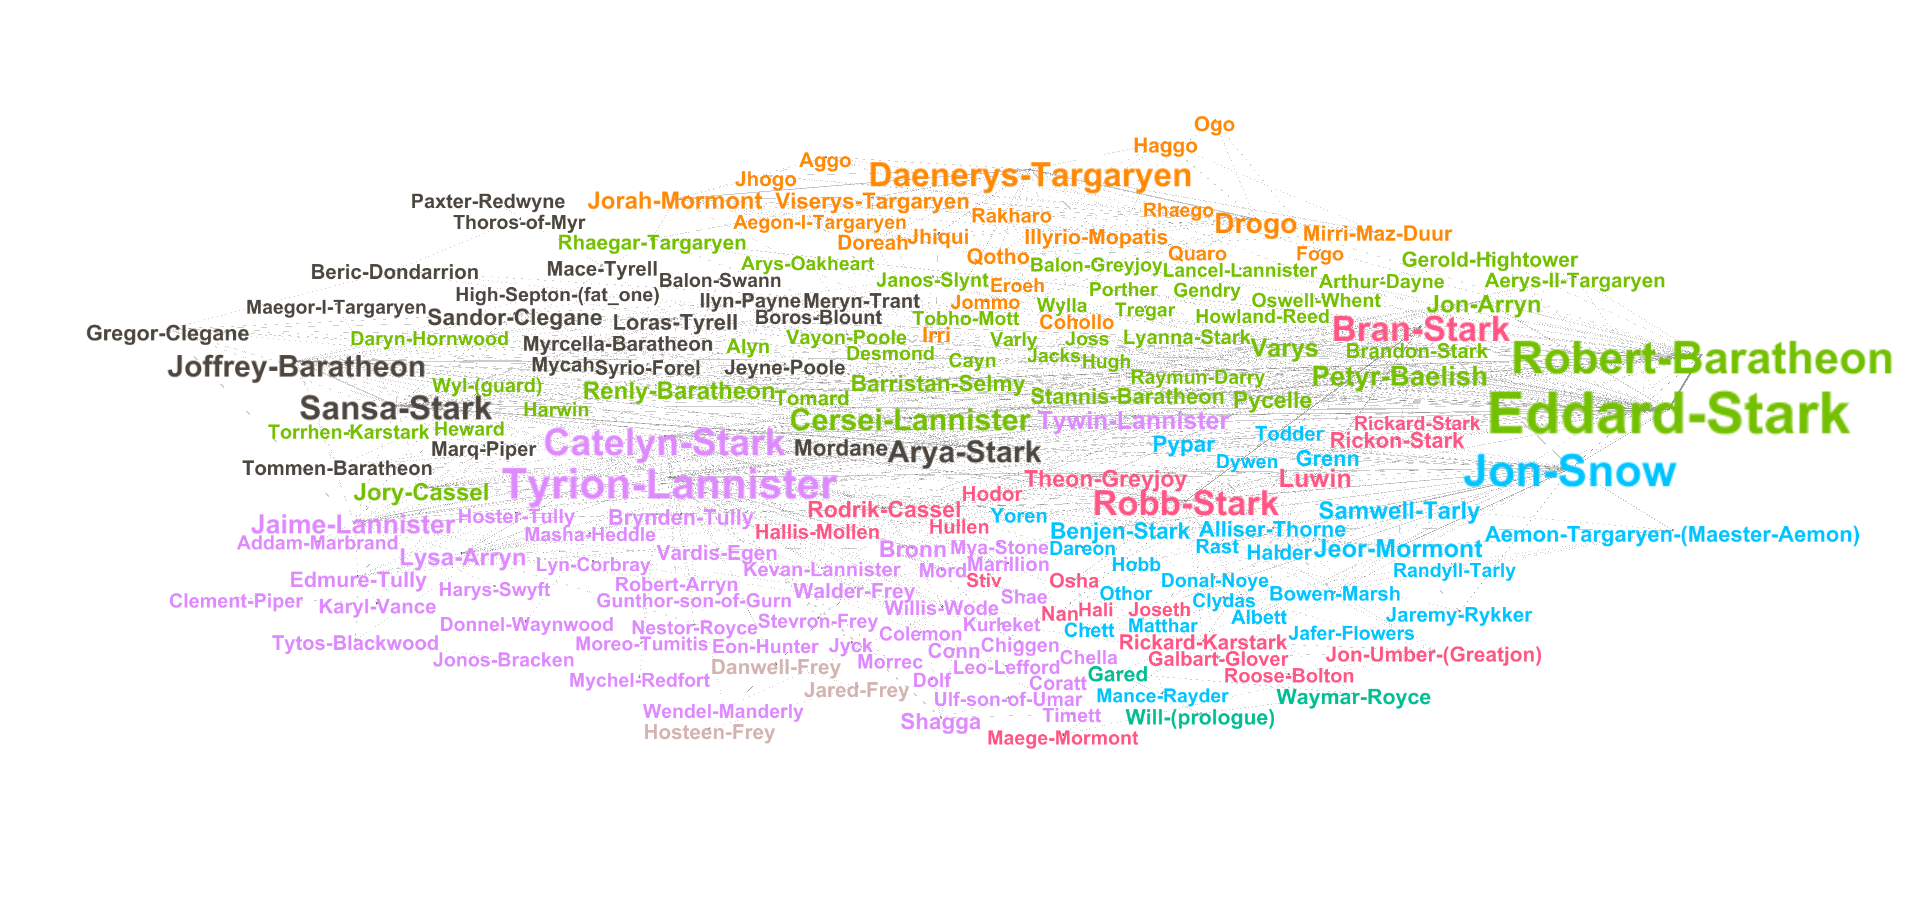
\includegraphics{b1.png}
\end{figure}

\newpage

\section{Libro 2}\label{libro-2}

\subsection{Moularidad, Pagerank y
Grafo}\label{moularidad-pagerank-y-grafo-1}

Modularity: 0.607 Modularity with resolution: 0.607 Number of
Communities: 7

\begin{figure}[htbp]  
\centering
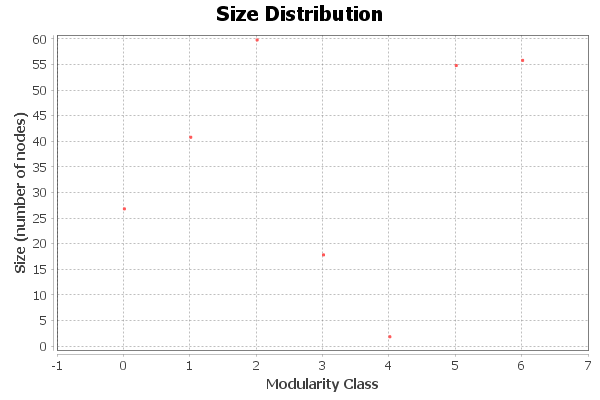
\includegraphics{modb2/communities-size-distribution.png}
\end{figure}

\begin{figure}[htbp]  
\centering
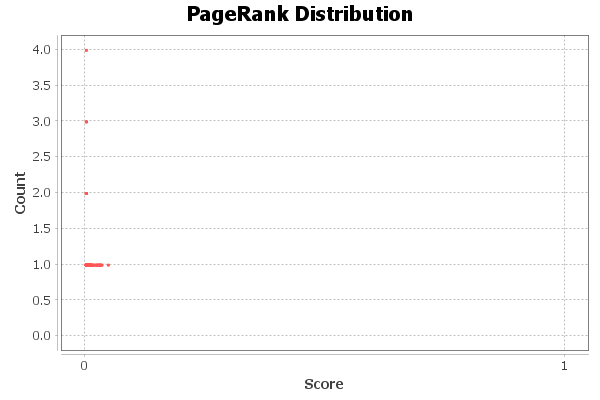
\includegraphics{prb2/pageranks.png}
\end{figure}

\begin{figure}[htbp]  
\centering
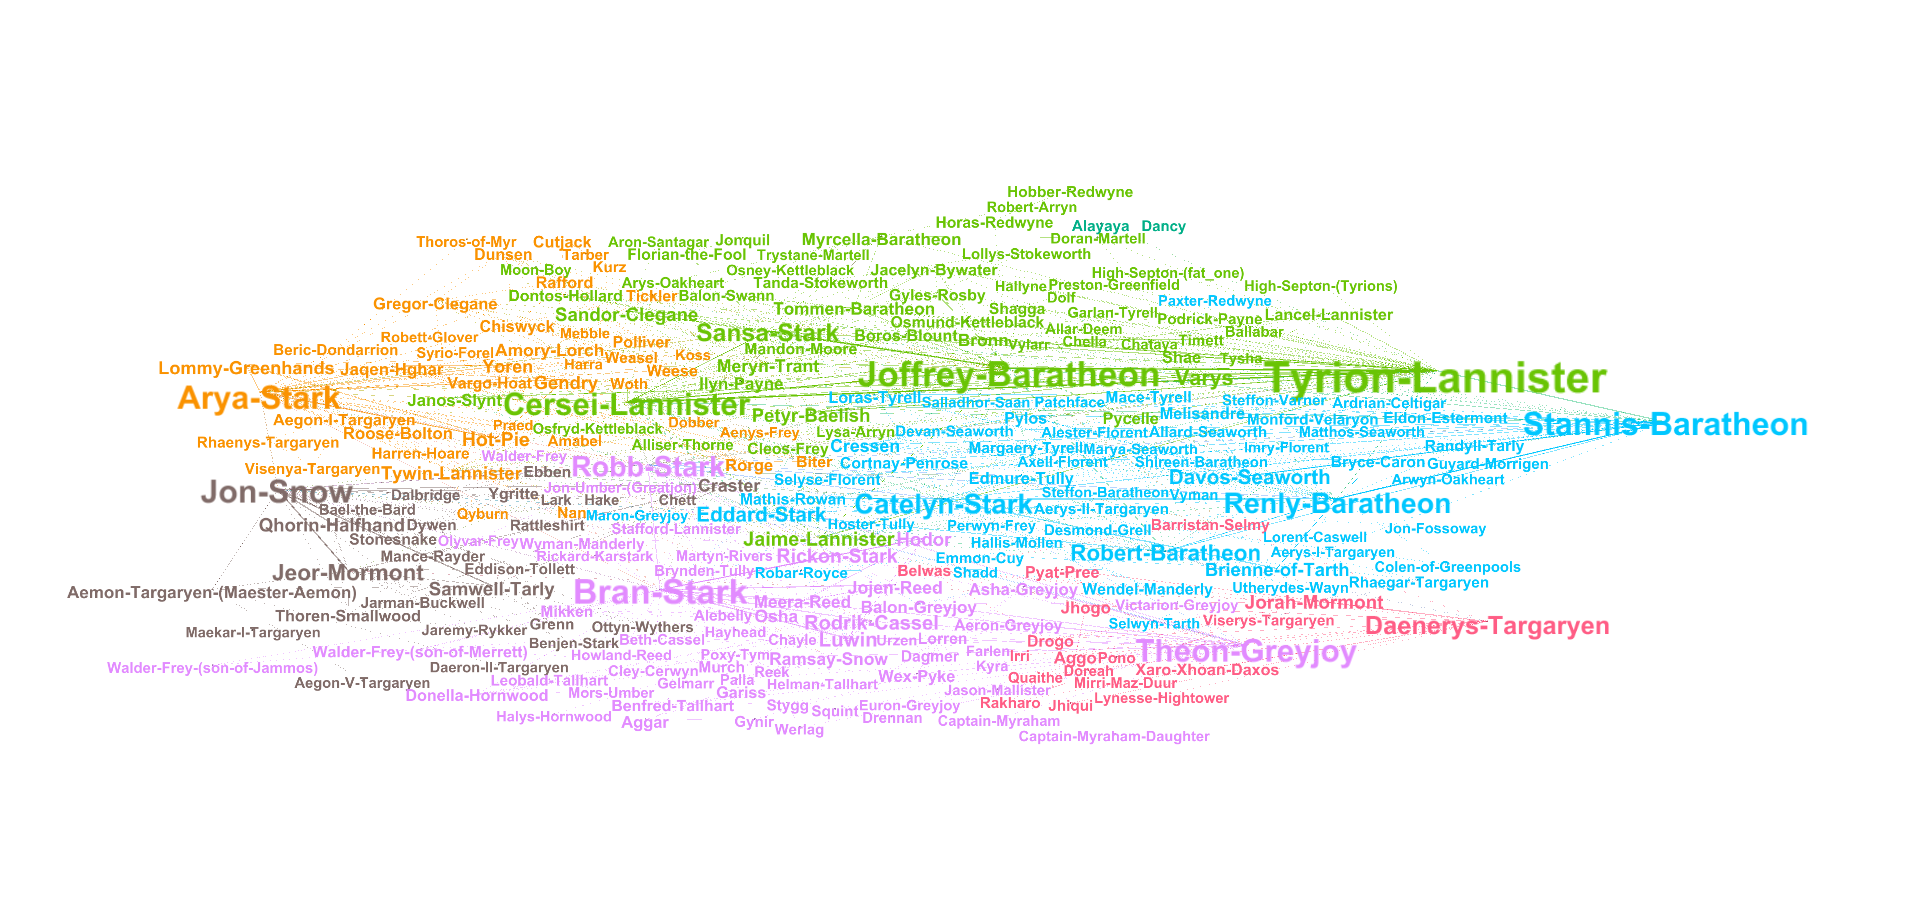
\includegraphics{b2.png}
\end{figure}\newpage

\section{Libro 3}\label{libro-3}

\subsection{Moularidad, Pagerank y
Grafo}\label{moularidad-pagerank-y-grafo-2}

Modularity: 0.649 Modularity with resolution: 0.649 Number of
Communities: 10

\begin{figure}[htbp]  
\centering
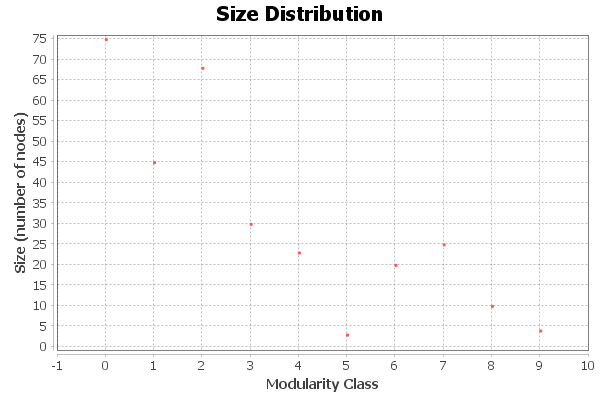
\includegraphics{modb3/communities-size-distribution.png}
\end{figure}

\begin{figure}[htbp]  
\centering
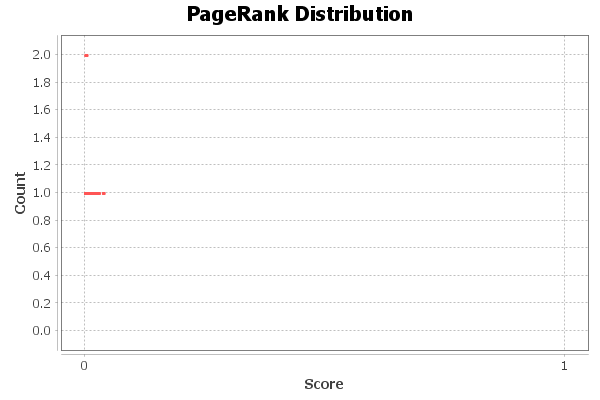
\includegraphics{prb3/pageranks.png}
\end{figure}

\begin{figure}[htbp]  
\centering
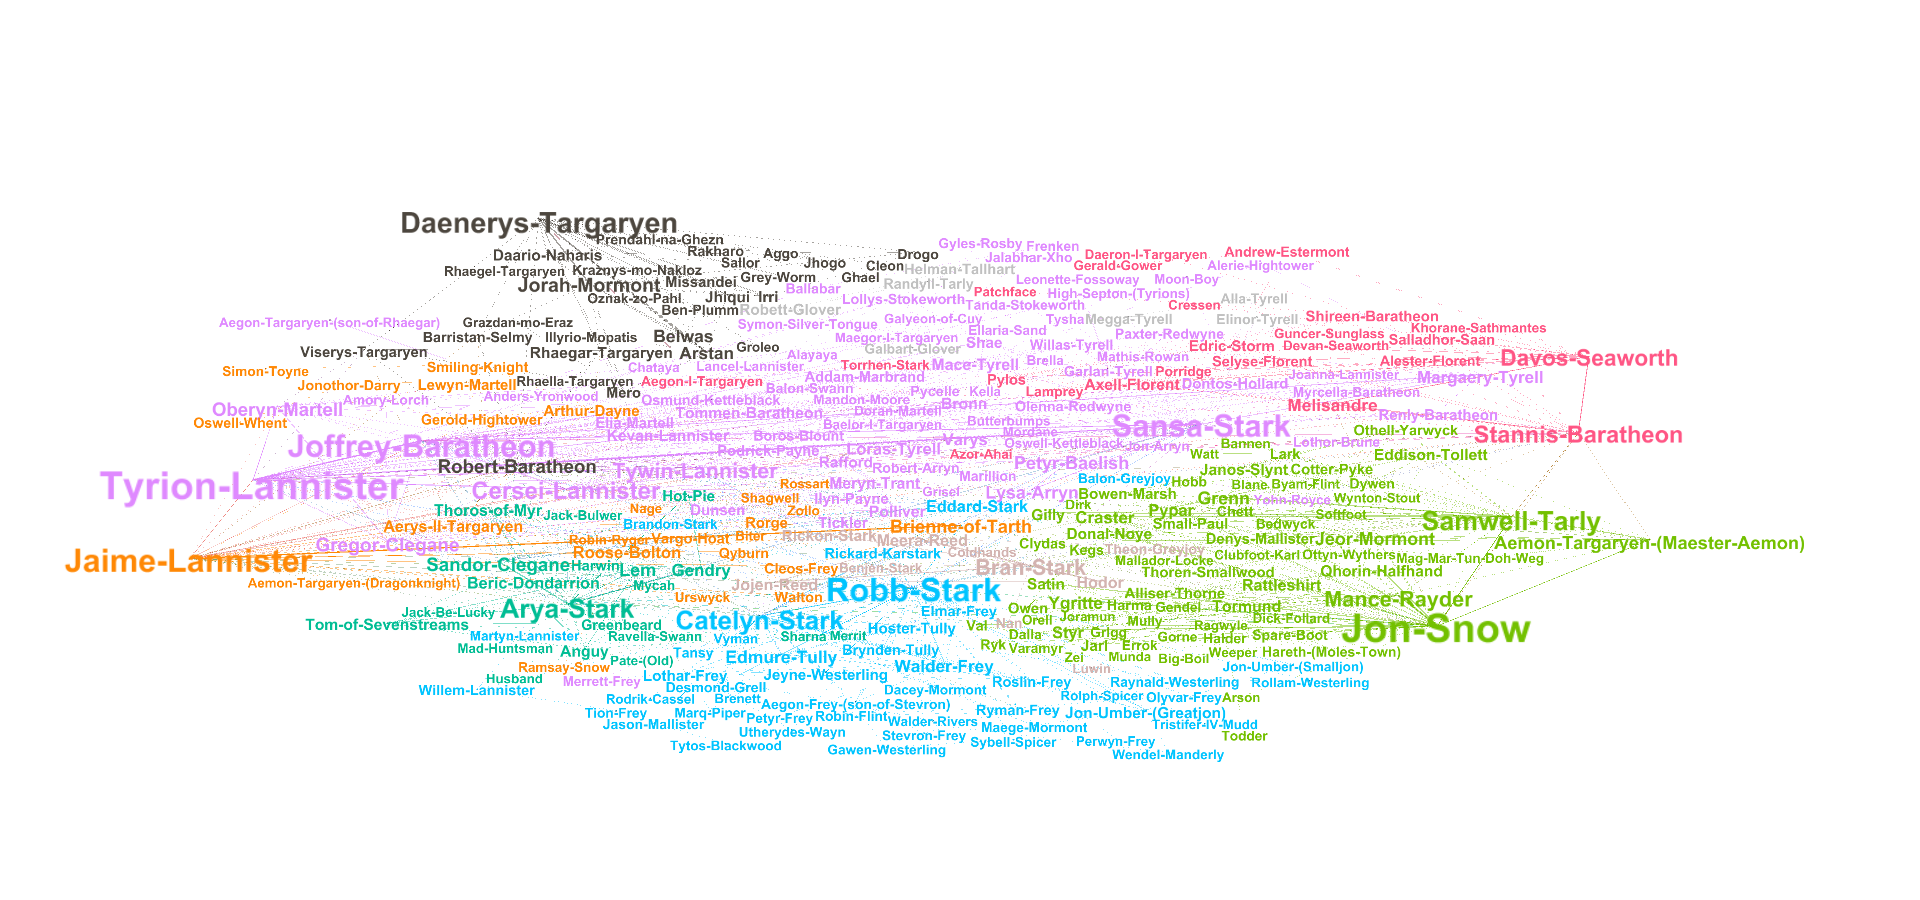
\includegraphics{b3.png}
\end{figure}\newpage

\section{Libro 4}\label{libro-4}

\subsection{Moularidad, Pagerank y
Grafo}\label{moularidad-pagerank-y-grafo-3}

Modularity: 0.665 Modularity with resolution: 0.665 Number of
Communities: 10

\begin{figure}[htbp]  
\centering
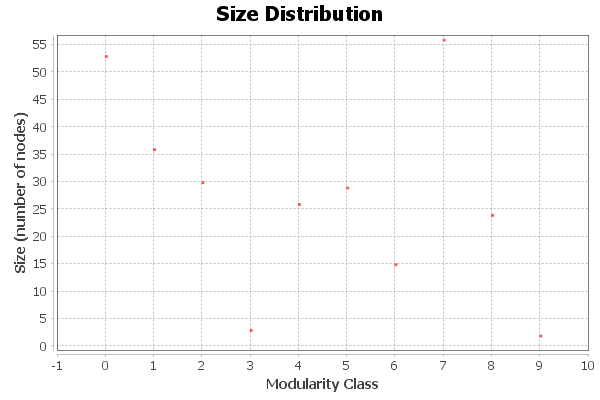
\includegraphics{modb4/communities-size-distribution.png}
\end{figure}

\begin{figure}[htbp]  
\centering
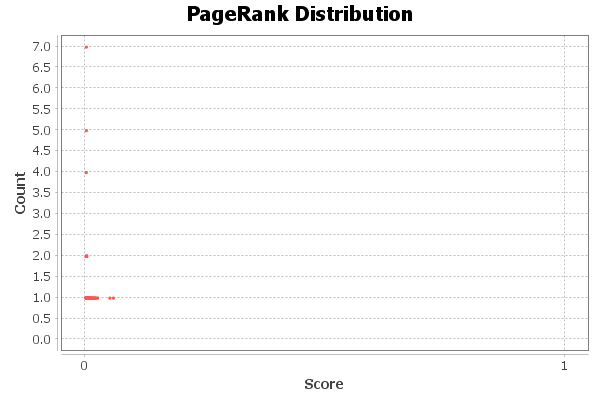
\includegraphics{prb4/pageranks.png}
\end{figure}

\begin{figure}[htbp]  
\centering
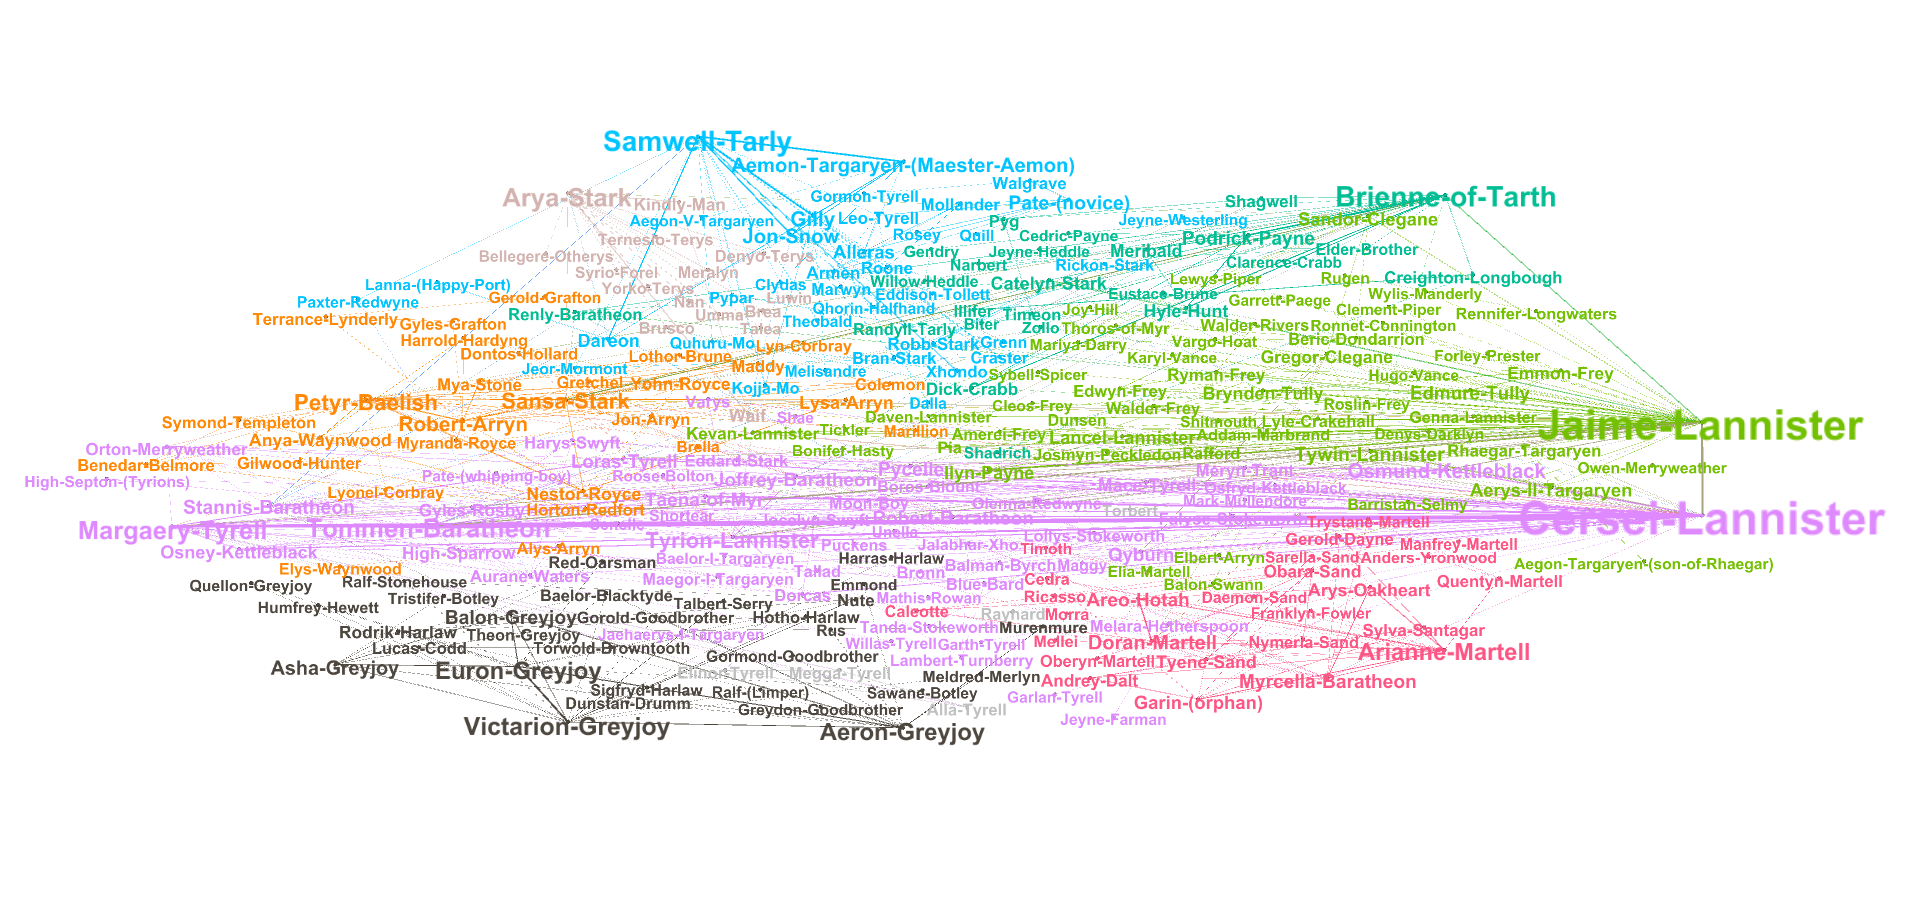
\includegraphics{b4.png}
\end{figure}\newpage

\section{Libro 5}\label{libro-5}

\subsection{Moularidad, Pagerank y
Grafo}\label{moularidad-pagerank-y-grafo-4}

Modularity: 0.704 Modularity with resolution: 0.704 Number of
Communities: 11

\begin{figure}[htbp]  
\centering
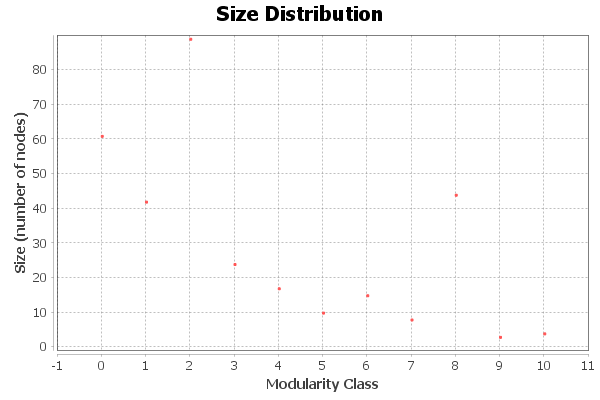
\includegraphics{modb5/communities-size-distribution.png}
\end{figure}

\begin{figure}[htbp]  
\centering
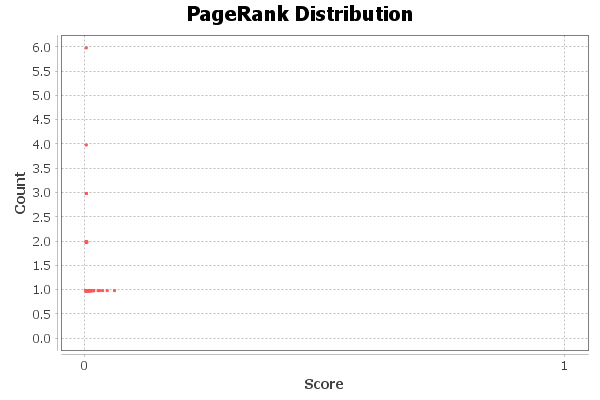
\includegraphics{prb5/pageranks.png}
\end{figure}

\begin{figure}[htbp]  
\centering
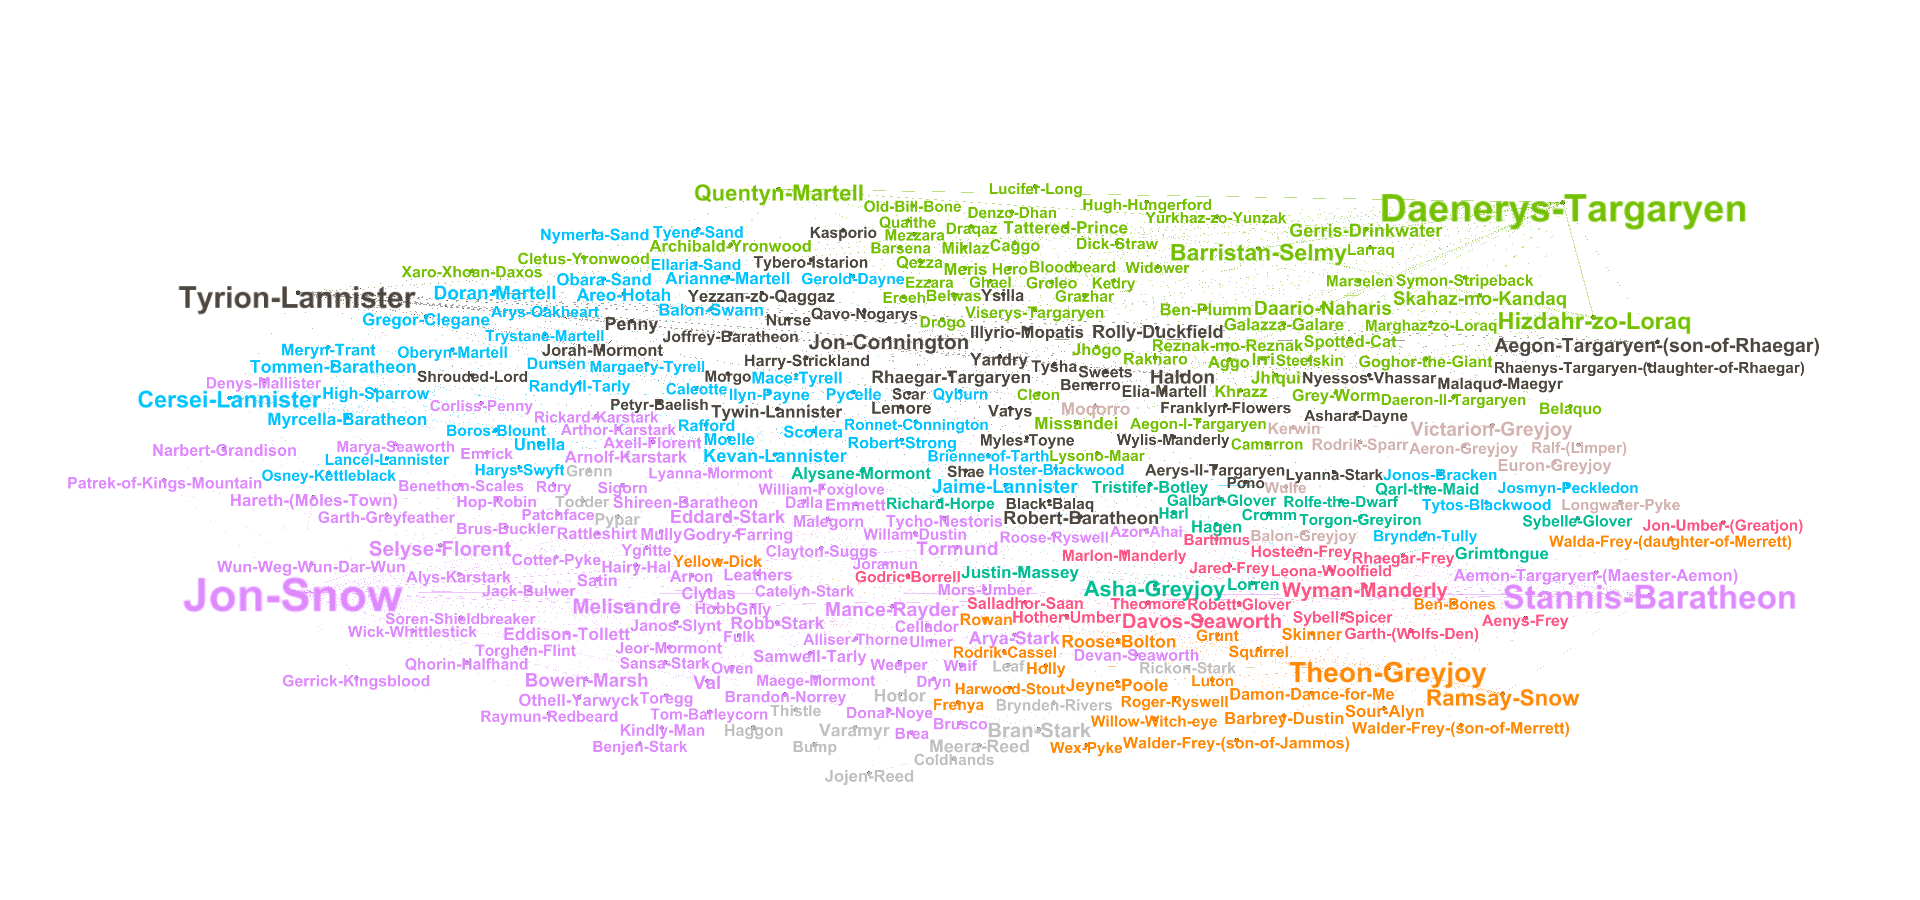
\includegraphics{b5.png}
\end{figure}


\end{document}
